% !TEX root = arbeit.tex
\section{Theory}

	\subsection{Requirements}
	% Mass, performance, Power consumption. (See latest references. Part of the introduction?)
	
	\subsection{Basic Theory about a TOF masspectrometry} % Allgemeine Theorie
	This chapter explains the function of a TOF instruments. A TOF mass spectrometer consists of, an ion-source, a mass analyser and a detector.\\
	In the ion source, the ions are produced and get all accelerated to the same energy.
	
	This is achieved by applying a high voltage pulse on the grid. % include a picture of a sample source.
	Depending on the initial position and velocity of the particles, they get a different amount of energy because they don't spend the same amount of time in the extraction field. These processes have a direct impact on the mass resolution. % Which?
	
	
	\subsection{Ion Optical Design, NIM specific elements} % ion source efficienies, reflectron double focusing, detector reflection of signal, signal matching. Density enhancement
	A time of flight mass spectrometer consists of, an ion-source, a mass analyser and a detector.\\
	
	\begin{figure}[htb] % Noch schauen, ob das noch verschoben wird.
		\centering
		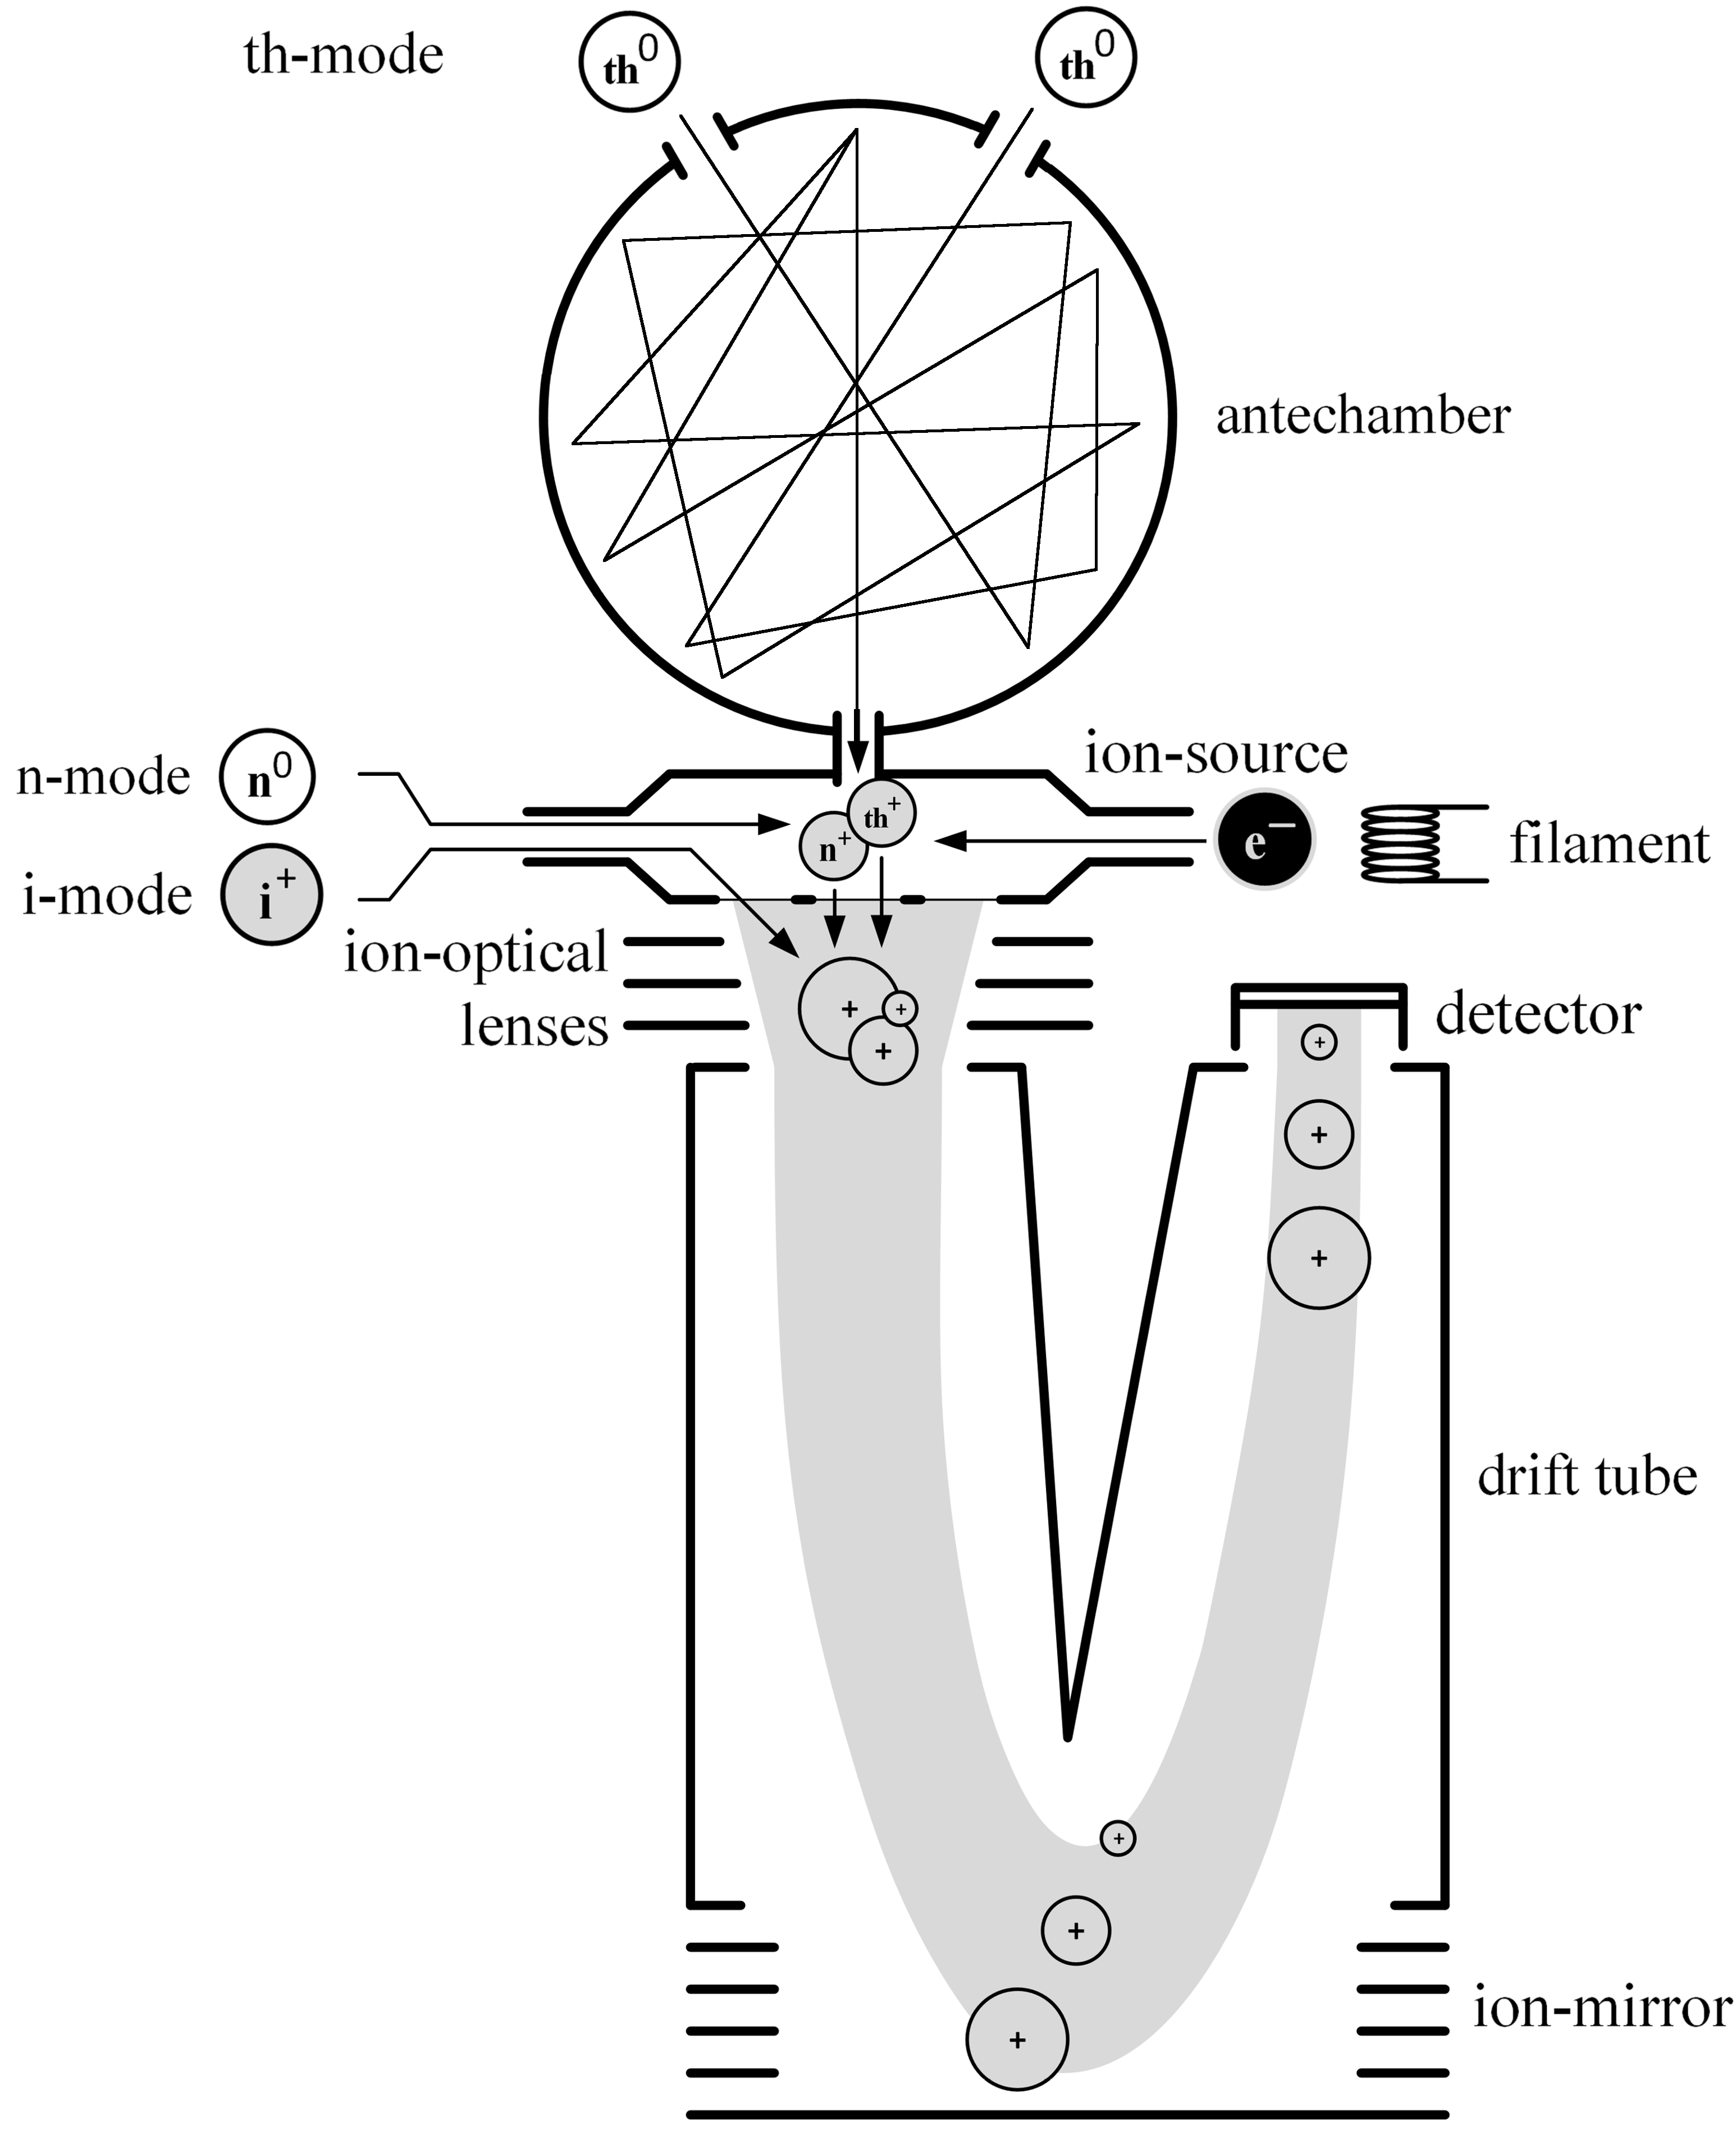
\includegraphics[width= 10cm]{Bilder/NIM_Sketch.png} % Bei Bild noch schauen, ob die Ränder drauf sind. Bei Zeiten noch Bild anpassen.
		\caption{Schematics of the NIM mass spectrometer. Adapted from \cite{Diss_Meyer}.}
		\label{fig:NIMSketch}
	\end{figure}

	%First overview and then go into the details.
	The NIM instrument is able to measure neutrals and ions. Neutral particles get ionised by electron ionisation. A filament is heated up until it emits electron. Ions enter the ion source directly.  % Noch genaue Formulierung nachschauen.
	All ions then get accelerated to the same energy and fly through the mass analyser. Light particles fly faster through the spectrometer than heavier ones. The different particle species arrive at different times at the detector. To enlarge the flight distance, an ion-mirror, which reflects the ions and leads them back to the detector. The used detector is a MCP detector. % Explain a little bit in more detail.
	
		\subsubsection{Ion-source}
		% More detailed explanation about the NIM ion source, function of the different specific electrodes. Or explain it later in detail when discussing the simulations in detail.
		To calculate the number of ions produced in the ion source we use:
		\begin{equation}
		I_{ion} = \beta\cdot Q_{ion}\cdot L\cdot n\cdot I_{em}
		\end{equation}
		With $\beta$ the extraction efficiency which is 1, % Noch schauen auf welchen Wert wir diese setzen wollen. 1= sehr gute Quelle, 0.01 = 1mus/100mus = Pulslänge Pulser/ Länge 1 Zyklus. Noch diskutieren, welche Werte beta haben kann oder einfach etwas setzen? Da die ersten Messresultate gut sind, würde ich eher auf 1 setzen.
		$L$ as the effective ionising path in our case 4~\si{\milli\metre}, $n$ the particle density, $I_{em}$ the electron emission current from the filament and $Q_{ion}$ the ionising cross section. The cross sections of species used in our calibration can be found in table % Ref. auf Tabelle und nur auf Stefans Diss verweisen oder die 4 Originalpaper zusammen suchen.
		
		
		
		% Reference: Bieler Diss 2012, Wurz 2011, Scherer 1999, Meyer 2013 Data Analysis, Wells 2011
		% Ionisation efficiency
		% Description of how it works with the energies. Electric -> kinetic. Pulser. E = 1/2 mv^2 = qU
		% Time focusing?
		% Mass calibration t/dt -> m/dm.
		% SNR definition. Picture?
		% Sensitivity estimation. Nessesary? If so, part of SNR discussion.
		% MCP detector. Gain calculation. How the detecotr works. Didn't do anything for further developement...
		% Antchamber. Explanation of closed and open source. Field of view. Densitiy enhancement.
	
	
\begin{comment}
	
	Explain how a TOF works. Source, reflectron, detector.
	Explanation of the antechamber at the end after explaining the different parts.
	
	Detection efficiency Ionsource, MCP? -> y-Achse
	Mass Analyser, mass spectrometer. Most important formulas. dm/m = dt/t...
	Sensitivity
	Density enhancement -> explanation about closed and open source
	Sketch of the instrument
	Requirements: Power, mass, mass resolution,... (At the end or at the beginning. Introduction)
	
	
	Ionisationseffizienz/ Ionenproduktion der wichtigsten Gase. Detektionseffizienz hängt auch von Effizienz der MCPs ab... Erklären weshalb man die Achsenskalieruing braucht (entweder Counts oder die angepasste a.u. bei der Fläche und Counts/s für das Spektrum)
	
\end{comment}
		